\documentclass[conference]{IEEEtran}
\IEEEoverridecommandlockouts

\usepackage{cite}
\usepackage{amsmath,amssymb,amsfonts}
\usepackage{graphicx}
\usepackage{textcomp}
\usepackage{xcolor}
\usepackage{booktabs}
\usepackage{multirow}
\usepackage{stfloats}
\usepackage[caption=false,font=footnotesize]{subfig}
\usepackage{url}
\usepackage[acronym,nomain,nonumberlist,nopostdot]{glossaries}

\renewcommand{\topfraction}{0.92}
\renewcommand{\bottomfraction}{0.75}
\renewcommand{\textfraction}{0.06}
\renewcommand{\floatpagefraction}{0.70}
\setcounter{topnumber}{3}
\setcounter{bottomnumber}{2}
\setcounter{totalnumber}{5}

\setacronymstyle{long-short}
\newacronym{dos}{DoS}{denial of service}
\newacronym{knn}{kNN}{k-nearest neighbours}
\newacronym{mcc}{MCC}{Matthews correlation coefficient}
\makenoidxglossaries
\renewcommand*{\glossarysection}[2][]{}

\begin{document}

\title{Classification of Network Traffic Attack Categories: A Tuned Random Forest Compared with k-Nearest Neighbours and Classification Trees}

\author{\IEEEauthorblockN{S.L. Johnson}
\IEEEauthorblockA{\textit{27356485}\\
\textit{Department of Computer Science}\\
\textit{Stellenbosch University}\\
27356485@sun.ac.za}
}

\date{}

\maketitle

\begin{abstract}
This study investigated ensemble learning for the classification of network
traffic into attack categories. A random forest was selected because the method
combines classification trees of the type used in a previous assignment. The forest was tuned
through a staged grid search, and further analyses examined the reasons behind the
observed performance. All models were evaluated under five-fold
stratified cross-validation on the folds of the previous assignment. The forest
tuned for macro-averaged F1 outperformed both previous models on that measure. A
bias--variance decomposition revealed that the previous classification tree was
heavily pruned, and removal of the pruning alone accounted for most of the gain
in macro-averaged F1. Ensembling reduced variance as theory predicts but improved
accuracy rather than macro-averaged F1. A forest tuned for the Matthews
correlation coefficient matched the macro-averaged F1 of the first forest at a
far higher accuracy.
\end{abstract}

%======================================================================
\section{Introduction}
%======================================================================

Network intrusion detection systems classify traffic records in order to
identify malicious activity, and classification models support that task by
assigning each record to an attack category. Moustafa and Slay constructed the
UNSW-NB15 dataset from a mixture of real normal traffic and synthetic attack
traffic \cite{moustafa2015}.

A previous assignment compared the \gls{knn} model with the classification tree
on a revised version of the dataset. The present report refers to that work as
assignment 2. The classification tree achieved the higher score under a
performance measure that weights every attack category equally.

The present study explores ensemble learning as a means of predicting
cyberattacks. An ensemble combines the predictions of several models into a
single prediction \cite{dietterich2000}, and the random forest is an ensemble of
classification trees \cite{breiman2001}. The random forest was chosen
deliberately because the forest uses the same type of tree and the same data
preparation as the classification tree of assignment 2. A comparison between the
forest and a single tree of the same configuration therefore isolates the
ensemble mechanism. A dissimilar ensemble method would change several factors at
once and obscure the source of any difference.

The purpose of the study was to determine whether a random forest outperforms the
models of assignment 2. Further analyses examined the source of any improvement,
the behaviour of the forest under tuning and the effect of class weighting.

The forest tuned for the primary measure outperformed both models of
assignment 2. A decomposition of the error into bias and variance then revealed
that the classification tree of assignment 2 was heavily pruned, so most of the
improvement over that tree arose from the absence of pruning in the forest. The
ensemble itself improved overall accuracy rather than the primary measure.

The remainder of the report is structured as follows. Section II provides
background on the models, on ensemble learning and on the dataset. Section III
describes the data preparation, the models and the implementation. Section IV
details the empirical procedure. Section V presents
and discusses the results, and Section VI concludes the study.

%======================================================================
\section{Background}
%======================================================================

This section provides the theoretical foundation for the study. The general
setting of supervised classification is introduced first, followed by the
performance measures and the decomposition of error into bias and variance. The
two models of assignment 2 are then described, followed by ensemble learning and
the random forest. The section closes with the treatment of class imbalance and
the data quality issues of the dataset.

\subsection{Supervised Classification}

An instance is one object to be classified. In the present study an instance is
one network flow, namely one connection between two hosts. Each instance is
described by a vector $\mathbf{x}$ of $d$ descriptive features and carries a
class label $y$ drawn from a set $C$ of $q$ classes. A training set $D$ is a
collection of $n$ labelled instances.

A classifier is a function $\hat{f}_D$ that maps a feature vector to a class
label, where the subscript indicates the training set used to construct the
classifier. The algorithm that constructs a classifier from a training set is
called a learning algorithm or learner. The quality of a single prediction is
measured by the zero-one loss, defined as
\begin{equation}
\ell\big(y, \hat{f}_D(\mathbf{x})\big) =
\begin{cases} 0 & \text{if } \hat{f}_D(\mathbf{x}) = y,\\ 1 & \text{otherwise.}\end{cases}
\end{equation}
The generalisation error of a classifier is the expected loss on instances not
seen during training \cite{hastie2009}. The training error is optimistic because
the classifier was fitted to the training instances. Performance is therefore
estimated on held-out instances throughout the study.

Hyperparameters are settings fixed before learning and are also called control
parameters. A hyperparameter shapes the class of rules that the learner is able to
represent, and tuning selects hyperparameter values through estimates of the
generalisation error.

\subsection{Performance Measures}

Let $\theta_c$ denote the number of true positives of class $c$, namely the
instances of class $c$ predicted as class $c$. Let $\xi_c$ denote the number of
false positives, namely the instances of other classes predicted as class $c$.
Let $\zeta_c$ denote the number of false negatives, namely the instances of class
$c$ predicted as another class. The precision and the recall of class $c$ are
given by
\begin{equation}
\pi_c = \frac{\theta_c}{\theta_c + \xi_c}, \qquad
\gamma_c = \frac{\theta_c}{\theta_c + \zeta_c} .
\end{equation}
Precision is the proportion of predictions of class $c$ that are correct, while
recall is the proportion of class $c$ that is detected. The F1 of class $c$ is the
harmonic mean of the two, given by
\begin{equation}
\eta_c = \frac{2\,\pi_c\,\gamma_c}{\pi_c + \gamma_c} ,
\end{equation}
so that $\eta_c$ is low when either component is low.

Macro-averaged F1 is the unweighted mean of $\eta_c$ over the $q$ classes and is
denoted $\bar{\eta}$. Every class therefore counts equally regardless of size.
Macro-averaged F1 was the primary measure in assignment 2 and remained the primary
measure in the present study. Macro-averaged precision and balanced accuracy are
the unweighted means of $\pi_c$ and $\gamma_c$ over the classes. Accuracy is the
proportion of all instances predicted correctly, namely $\sum_{c} \theta_c / n$.
Accuracy therefore counts every instance equally and is dominated by the large
classes.

The \gls{mcc} measures the correlation between predicted and true labels, and
Gorodkin defined the multi-class form used in the present study
\cite{gorodkin2004}. With $\hat{n}_c$ the number of instances predicted as class
$c$, the multi-class \gls{mcc} is given by
\begin{equation}
\varphi = \frac{n \sum_{c} \theta_c - \sum_{c} \hat{n}_c\, n_c}
{\sqrt{\big(n^2 - \sum_{c} \hat{n}_c^2\big)\big(n^2 - \sum_{c} n_c^2\big)}} ,
\end{equation}
where a value of one indicates perfect prediction and a value of zero indicates
no better than chance. Like accuracy, the \gls{mcc} counts every instance equally
and therefore represents the opposite value judgement to macro-averaged F1.

\subsection{Bias and Variance}

The training set is a random sample, so a different sample produces a different
classifier with different predictions at the same feature vector $\mathbf{x}$.
Domingos decomposed the expected zero-one loss at $\mathbf{x}$ into terms that
describe this behaviour \cite{domingos2000}.

Let $y_*$ denote the optimal prediction at $\mathbf{x}$, namely the most probable
class. Let $\bar{y}$ denote the main prediction, namely the class predicted most
often across training sets. The bias at $\mathbf{x}$ is given by
\begin{equation}
\beta(\mathbf{x}) = \ell(y_*, \bar{y}),
\end{equation}
so the bias equals one when the main prediction is wrong. The variance at
$\mathbf{x}$ is given by
\begin{equation}
\nu(\mathbf{x}) = \mathbb{E}_D\big[\ell\big(\bar{y}, \hat{f}_D(\mathbf{x})\big)\big],
\end{equation}
where $\mathbb{E}_D$ denotes the expectation over training sets. The variance is
therefore the probability that a single classifier disagrees with the main
prediction.

The noise is the expected loss of the optimal prediction and is unavoidable for
every classifier. Domingos showed that the expected loss equals a
weighted noise term plus the bias plus $\kappa\,\nu(\mathbf{x})$ \cite{domingos2000}. The coefficient
$\kappa$ equals one when the main prediction is correct and is negative when the
main prediction is wrong. Variance therefore adds to the loss on instances
predicted correctly on average. On instances predicted incorrectly on average,
variance reduces the loss because a classifier that disagrees with a wrong main
prediction is sometimes correct.

Capacity is the ability of a model to represent complex rules. A model with high
capacity tends towards low bias and high variance, while a model with low capacity
tends towards high bias and low variance \cite{hastie2009}.

\subsection{k-Nearest Neighbours}

The \gls{knn} rule assigns a query instance to the class most heavily represented
among the $k$ training instances closest to the query \cite{cover1967}. The
training set therefore constitutes the model, and all computation is deferred to
prediction time.

Closeness is measured by a distance function. With $\mathbf{z}$ a second feature
vector, the Minkowski distance of order $\lambda$ between $\mathbf{x}$ and
$\mathbf{z}$ is given by
\begin{equation}
\delta_\lambda(\mathbf{x}, \mathbf{z}) = \Big( \sum_{j=1}^{d} |x_j - z_j|^\lambda \Big)^{1/\lambda},
\end{equation}
where $x_j$ and $z_j$ denote the $j$-th components of $\mathbf{x}$ and
$\mathbf{z}$. The order $\lambda = 2$ yields the Euclidean distance, while
$\lambda = 1$ yields the Manhattan distance that grows more slowly with a large
difference in a single component. Under distance weighting, each neighbour casts
a vote weighted by the inverse of the distance to the query.

A decision boundary separates the regions of the feature space assigned to
different classes. The neighbourhood size $k$ controls the capacity of the model \cite{hastie2009}.
A small value of $k$ produces a boundary that follows individual instances, while
a large value produces a smooth boundary. Two further properties follow from the
reliance on distance. A feature with a large numeric range dominates the
distance, and redundant features contribute one underlying quantity more than
once.

\subsection{Classification Trees}

A classification tree predicts through a sequence of yes-or-no questions. Each
question tests whether one feature lies below a threshold and sends the instance
to one of two branches. A point in the tree where a question is asked is called a
node, and the questions continue until the instance reaches a leaf that carries a
class prediction.

Hastie \textit{et al.} described the construction of such trees through recursive
binary splitting \cite{hastie2009}. At each node the algorithm selects the feature and threshold
that most reduce impurity, a measure of how mixed the classes in a node are. With
$p_c$ the proportion of class $c$ among the training instances in a node, the
Gini impurity of the node is given by
\begin{equation}
g = 1 - \sum_{c \in C} p_c^2
\end{equation}
as given by Hastie \textit{et al.} \cite{hastie2009}. The entropy of the node
is given by
\begin{equation}
h = -\sum_{c \in C} p_c \log_2 p_c
\end{equation}
as used by Quinlan \cite{quinlan1986}. Both measures equal zero for a node that
contains a single class and are largest when the classes are evenly mixed. Growth
stops when a node is pure or when a split would leave fewer instances in a leaf
than the minimum leaf size $\omega$.

A tree grown until every leaf is pure reproduces the training sample exactly,
including noise. Cost-complexity pruning removes a branch when the improvement
from the branch does not justify the size of the branch \cite{hastie2009}. With
$r$ the training misclassification cost of a tree and $l$ the number of leaves,
the pruned tree minimises
\begin{equation}
r_\alpha = r + \alpha\, l ,
\end{equation}
where $\alpha \geq 0$ is the complexity parameter. Each leaf must justify the cost
$\alpha$, so a larger value of $\alpha$ yields a smaller tree with fewer leaves and
a lower capacity.

A threshold test is invariant under any strictly increasing transformation of the
feature tested, because the transformation preserves the order of the values. A
tree is therefore unaffected by the numeric range of a feature. Breiman identified
classification trees as unstable, meaning that a small change in the training data
produces a large change in the tree \cite{breiman1996}. A change in an early split
alters every node below the split, so a fully grown tree has low bias and high
variance.

\subsection{Ensemble Learning and Random Forests}

An ensemble combines the predictions of several models, and Dietterich identified
three reasons why an ensemble often outperforms the individual members
\cite{dietterich2000}. The statistical reason is that averaging hedges against an
unlucky choice among equally good models. The computational reason concerns
greedy learners. A greedy learner makes the best choice at each step without
look-ahead and is therefore liable to stop at a local optimum, namely a solution
that no small change improves. A tree is a greedy learner because the tree selects each
split in turn, and different runs of a greedy learner reach different local
optima. The representational reason is that a combination represents decision
boundaries beyond the reach of any single member.

Averaging reduces variance. Let $m$ denote the number of models, and let
$\hat{f}_b(\mathbf{x})$ denote the prediction of model $b$. If each prediction has
variance $\sigma^2$ and each pair of predictions has correlation $\rho$, the
variance of the average prediction is given by
\begin{equation}
\operatorname{Var}\Big(\frac{1}{m}\sum_{b=1}^{m} \hat{f}_b(\mathbf{x})\Big)
= \rho\,\sigma^2 + \frac{1-\rho}{m}\,\sigma^2 ,
\end{equation}
where $\operatorname{Var}$ denotes the variance over training sets
\cite{hastie2009}. The second term vanishes as $m$ grows, so additional models
never increase the variance. The first term remains as a floor on the variance,
and only a reduction in the correlation $\rho$ lowers that floor.

The name bagging is short for bootstrap aggregating, a method that creates variety
through bootstrap samples \cite{breiman1996}. A bootstrap sample draws $n$
instances with replacement from the $n$ available. A given instance is missed by
all $n$ draws with probability $(1 - 1/n)^n$, a value that tends to
$e^{-1} \approx 0.368$ as $n$ grows. Here $e$ denotes the base of the natural
logarithm, so each bootstrap sample contains about 63.2 percent of the distinct
instances. Bagging trains one model on each bootstrap sample and averages the
predictions.

The base learner of an ensemble is the type of model that the ensemble combines. A
random forest uses classification trees as base learners and adds a second source
of variety \cite{breiman2001}. Each tree considers only a random subset of $a$
features at every split, and the trees are grown without pruning. Without the
random subsets, every tree would select the same dominant features near the root
and the trees would be highly correlated. The setting $a = d$ reduces the random
forest to bagging. The implementation used in the present study combines the
trees through soft
voting.\footnote{\url{https://scikit-learn.org/stable/modules/ensemble.html}}
Soft voting averages the class proportions in the leaves reached by the trees and
predicts the class with the largest average.

Breiman quantified the trade-off in the choice of $a$ \cite{breiman2001}. The
margin $\mu(\mathbf{x}, y)$ is the proportion of trees that vote for the true class
minus the largest proportion that vote for any other class. The raw margin of a single tree is one for a vote for the true class,
minus one for a vote for the strongest other class and zero otherwise. The
strength $s$ is the expected margin, and the mean correlation $\bar{\rho}$ is the
mean correlation between the raw margins of pairs of trees. Breiman showed that the generalisation error
$\psi$ of the forest is bounded by
\begin{equation}
\psi \leq \bar{\rho}\,\frac{1 - s^2}{s^2} .
\end{equation}
Breiman observed that the correlation rises steadily as $a$ grows, while the
strength stops rising beyond a small value of $a$ \cite{breiman2001}. The best value
of $a$ therefore balances the two effects.

Boosting is the main alternative family of ensembles. Freund and Schapire showed
that boosting builds a strong classifier from a sequence of weak classifiers
\cite{freund1997}, where a weak classifier performs only slightly better than
chance. Each classifier in the sequence concentrates on the instances
misclassified by the earlier classifiers. Boosting therefore targets weak
classifiers with high bias, whereas the random forest targets strong classifiers with high variance such as
fully grown trees \cite{hastie2009}.

\subsection{Class Imbalance}

A class distribution is imbalanced when the classes differ greatly in size. He and
Garcia reported that a learner that minimises the overall error rate tends to neglect
the small classes \cite{he2009}. One remedy is cost-sensitive learning, an approach
that assigns a higher cost to errors on the small classes.

Class weighting is a form of cost-sensitive learning. With $n_c$ the number of
instances of class $c$, the balanced weighting of the implementation used in the
present study assigns class $c$ the weight
\begin{equation}
w_c = \frac{n}{q\, n_c}
\end{equation}
so that every class carries the same total
weight.\footnote{\url{https://scikit-learn.org/stable/modules/generated/sklearn.utils.class_weight.compute_class_weight.html}}
In a tree, each instance counts with the weight of the class of the instance in
both the impurity and the prediction of each leaf.

\subsection{Data Quality Issues}

The revised dataset contains 257\,673 instances, 42 descriptive features and 10
classes. Of the 42 features, 39 are numeric and three are nominal. A nominal
feature takes category names as values. The three nominal features are the
transaction protocol, the service and the connection state. The dataset has five
data quality issues relevant to the present study.

First, the class distribution is imbalanced. The Normal class holds 93\,000
instances against 174 for the Worms class, a ratio of 534 to 1.
Table~\ref{tab:classes} reports the full distribution.

\begin{table}[t]
\centering
\caption{Class distribution, conflict rate and idealised ceiling}
\label{tab:classes}
\small
\begin{tabular}{lrrr}
\toprule
Class & Instances & Conflicting & Ceiling F1 \\
\midrule
Normal & 93\,000 & 0.010 & 0.996 \\
Generic & 58\,871 & 0.006 & 0.997 \\
Exploits & 44\,525 & 0.371 & 0.813 \\
Fuzzers & 24\,246 & 0.149 & 0.924 \\
Denial of service & 16\,353 & 0.774 & 0.549 \\
Reconnaissance & 13\,987 & 0.161 & 0.914 \\
Analysis & 2\,677 & 0.770 & 0.375 \\
Backdoor & 2\,329 & 0.849 & 0.265 \\
Shellcode & 1\,511 & 0.009 & 0.997 \\
Worms & 174 & 0.086 & 0.955 \\
\bottomrule
\end{tabular}
\end{table}

Second, the numeric ranges differ by many orders of magnitude. The source load
feature reaches $5.99 \times 10^{9}$ while the transaction depth feature reaches
only 172. Third, 12 pairs of numeric features have a Pearson correlation of at least
0.95 in absolute value. Pearson correlation measures the strength of the linear
relationship between two features on a scale from $-1$ to 1. Fourth, the service
feature is missing for 141\,321 instances.

Fifth, many instances are exact duplicates. The 257\,673 instances contain only
153\,684 distinct feature vectors, and 46.5 percent of instances share a feature
vector with another instance. More seriously, 40\,400 instances share a feature
vector with an instance of a different class. The column ``Conflicting'' of
Table~\ref{tab:classes} gives the proportion of each class affected, a proportion
that reaches 0.849 for Backdoor and 0.774 for \gls{dos}.

Instances with identical features and different labels set a floor on the error
of every classifier. A classifier assigns one label to all instances with the same
feature vector, so at least one of the conflicting instances is misclassified.
Label noise refers to incorrect class labels. Fr\'enay and Verleysen
identified insufficient information in the description of an instance as one source
of label noise \cite{frenay2014}. The conflicting instances fit that source,
because the 42 features fail to distinguish the classes involved.

The size of the floor was estimated through an idealised ceiling classifier that
memorises every instance. For each group of identical feature vectors, the ceiling
classifier predicts the most frequent label of the group. The ceiling classifier
achieved an accuracy of 0.914, and the column ``Ceiling F1'' of
Table~\ref{tab:classes} reports the per-class F1. The ceiling is optimistic
because the ceiling classifier is evaluated on the instances memorised.

In summary, the trees and the forest require only a numeric encoding of the nominal
features. The \gls{knn} model additionally requires scaling and the removal of
redundant features. No model is able to separate the conflicting instances. The
\gls{dos}, Analysis and Backdoor classes therefore have low ceilings for every
model.

%======================================================================
\section{Methodology}
%======================================================================

This section describes the treatment of the dataset and the construction of the
models. The data preparation common to all models is described first, followed by
the pre-processing specific to each family of models. The section closes with the
model configurations and the implementation.

\subsection{Data Preparation}

The dataset was read with the character ``?'' treated as a missing value marker.
The identifier feature was removed for every model. A unique identifier allows a
tree to isolate single instances and adds an uninformative dimension to every
distance.

Missing values in the service feature were recorded as a separate category named
``none''. The feature description supplied with the dataset records a service only
when the service is commonly used, so a missing service indicates an uncommon
service. The absence is itself informative, and imputation would destroy that
information.

The login feature for the file transfer protocol is documented as binary. The
feature nonetheless held the value 2 for 10 instances and the value 4 for 16
instances, and the irregular values were clipped to the interval $[0, 1]$. No
numeric value was missing and no feature was constant. Duplicate instances were
retained so that every model used the same instances as assignment 2.

\subsection{Pre-processing for k-Nearest Neighbours}

The \gls{knn} pipeline of assignment 2 was retained unchanged. A pipeline is a
sequence of transformations followed by a model and is fitted as one unit. Four
transformations addressed the issues identified in Section II.

The 12 correlated pairs form six groups of features that each describe one
quantity. One representative of each group was retained, so nine features were
removed. The retained byte counts were \texttt{sbytes} and \texttt{dbytes}, and the
retained window feature was \texttt{swin}. The retained connection counters were
\texttt{ct\_srv\_src} and \texttt{ct\_dst\_ltm}, and the retained login feature was
\texttt{is\_ftp\_login}. Every pair of features within a group is correlated at 0.95
or above, so the choice of representative has little effect on the distance.

A logarithmic transformation of the form $\log(1+x)$ was then applied to every
numeric feature. Every numeric value in the dataset is non-negative, so the
transformation is defined everywhere. The transformation compresses the large
values while preserving the order of the values.

Each numeric feature was then scaled. Standardisation subtracts the mean and
divides by the standard deviation, a measure of spread around the mean. Robust
scaling subtracts the median and divides by the interquartile range, namely the
width of the middle half of the values. Extreme values therefore have little effect
on robust scaling. The tuning of assignment 2 selected robust scaling.

The three nominal features were one-hot encoded. One-hot encoding replaces a
nominal feature by one binary feature per category, and categories with a relative
frequency below 0.01 were merged into a single infrequent category. An integer code
would impose an order and a distance between categories that do not exist. Wilson
and Martinez proposed heterogeneous distance functions that treat nominal features
directly \cite{wilson1997}. One-hot encoding was preferred because the resulting
space of 48 features admits a single Minkowski distance for all features.

\subsection{Pre-processing for the Tree-Based Models}

The classification trees and the random forests received a single transformation.
The three nominal features were ordinal encoded because the implementation of the
trees requires numeric input. Ordinal encoding replaces each category by an
integer and so imposes an arbitrary order on the categories. A tree still isolates
any single category through two threshold tests, so the arbitrary order costs at
most additional depth. The invariance argument of Section II makes scaling and
logarithmic transformation unnecessary.

\subsection{Model Configurations}

Six models were compared. The \gls{knn} model of assignment 2 used robust scaling
and distance weighting with $\lambda = 1$ and $k = 3$. The classification tree of
assignment 2 used the Gini impurity without class weighting or depth limit, with
$\omega = 1$ and $\alpha = 10^{-4}$.

The untuned forest used the default settings of the implementation, namely 100
trees with the Gini impurity and no class weighting. The untuned forest also used
$\omega = 1$ and $a = 6$, the square root of $d$ rounded
down.\footnote{\url{https://scikit-learn.org/stable/modules/generated/sklearn.ensemble.RandomForestClassifier.html}}
Two tuned forests were constructed through a staged grid search. The first forest
was selected by macro-averaged F1 and the second by the \gls{mcc}.

The sixth model is the classification tree of assignment 2 without pruning, namely
with $\alpha = 0$. The unpruned tree was added after the decomposition into bias
and variance revealed the extent of the pruning. The
unpruned tree is the base learner of the random forest, so a comparison with the
unpruned tree separates the effect of ensembling from the effect of pruning.

\subsection{Implementation}

All models were implemented in Python.\footnote{\url{https://www.python.org}} The
scikit-learn library provided the models, the transformations and the
cross-validation procedure \cite{pedregosa2011}. The library was selected because
one library implements all three model families behind a common interface. Every
model therefore received identical data splits and identical evaluation code. The
pandas library provided the data
structures,\footnote{\url{https://pandas.pydata.org}} and the NumPy library
provided the numerical routines.\footnote{\url{https://numpy.org}} The SciPy library
provided the statistical tests,\footnote{\url{https://scipy.org}} and the Matplotlib
library provided the figures.\footnote{\url{https://matplotlib.org}}

Each model was a single pipeline fitted within each training partition, so no
transformation was fitted on data used for evaluation. The predictions of the
\gls{knn} model were taken from assignment 2 rather than recomputed. Prediction with
the \gls{knn} model requires about $10^{10}$ distance computations per fold because
every test instance is compared with every training instance. The model is
deterministic, so a refit would reproduce the saved predictions. The classification
tree of assignment 2 was refitted and reproduced the predictions of assignment 2 on
all 257\,673 instances. The data and the partitions were therefore identical to
those of assignment 2.

In summary, every tree-based model shared one pre-processing step. Differences
among the trees and forests therefore arise from the learning mechanism and the
configuration alone.

%======================================================================
\section{Empirical Procedure}
%======================================================================

This section describes the procedure followed to obtain the results. The
cross-validation protocol is described first, followed by the tuning procedure. The
analyses that explain the results then follow, and the section closes with the
statistical analysis.

\subsection{Cross-Validation Protocol}

Performance was estimated through $v$-fold cross-validation \cite{hastie2009}
with stratified folds. The dataset is partitioned into $v$ folds. Each fold serves once
as the test partition while the remaining folds form the training partition.
Every instance is therefore predicted once by a model that did not see the
instance. Stratification preserves the class distribution in every fold, and
without stratification a fold could contain almost no Worms instances.

Five folds were used, as in assignment 2. The folds were generated from the random
seed of assignment 2, a number that fixes the sequence of random numbers used to
form the folds. Every model was therefore evaluated on identical partitions, so
the scores of any two models on the same fold are paired. The evaluation on the
five folds is referred to as the outer cross-validation.

\subsection{Tuning Procedure}

The forest was tuned through a staged grid search. A grid search evaluates every
combination of the candidate values, while a staged search fixes the winner of one
small grid before the next grid is searched. The staged search is cheaper but
assumes little interaction between stages. Hyperparameters expected to interact
were therefore searched in the same stage, and each stage was designed to reveal one
aspect of the behaviour of the forest.

Each candidate was evaluated by five-fold cross-validation within the tuning data,
referred to as the inner cross-validation. The tuning data was the stratified
subsample of 40\,000 instances used by assignment 2, so the forest received the same
tuning budget as the models of assignment 2. Table~\ref{tab:search} reports the
search space and the selected values.

\begin{table}[t]
\centering
\caption{Search space and selected configurations of the random forest}
\label{tab:search}
\small
\begin{tabular}{llll}
\toprule
Parameter & Values & \multicolumn{2}{c}{Selected for} \\
& & Macro F1 & \acrshort{mcc} \\
\midrule
$a$ & 1, 6, 10, 21, 42 & 21 & 21 \\
Weighting & none, balanced, & balanced & none \\
& balanced per tree & & \\
$\omega$ & 1, 2, 5, 10, 25 & 2 & 10 \\
Impurity & Gini, entropy & entropy & entropy \\
$m$ & 1 to 500 & 100 & 50 \\
\bottomrule
\end{tabular}
\end{table}

The first stage measured how much decorrelation benefits the forest and whether
class weighting helps the small classes. The two hyperparameters were searched
together because weighting changes the splits that appear best. The values of $a$
span the full range from one feature to all 42 features, with the default of 6 and
the values 10 and 21 filling the gap. The weighting options are the three options of
the implementation, and the option ``balanced per tree'' recomputes the weights on
each bootstrap sample.

The second stage crossed $\omega$ with the impurity measure to establish whether the
trees of a forest should be fully grown. The values of $\omega$ run from fully grown
trees to clearly restrained trees in roughly doubling steps. Both stages used 200
trees so that the randomness of a small forest did not decide the comparison.

The number of trees was not tuned in the usual sense, because Breiman showed that
the error of a random forest converges as trees are added \cite{breiman2001}. A
forest of 500 trees was therefore grown once per inner fold. A forest of $m$ trees
equals the average of the first $m$ trees of the larger forest, so every forest of
up to 500 trees was scored from a single fit. The smallest forest within 0.002 of
the 500-tree score was selected. The tolerance lies below the fold-to-fold standard
deviation of 0.0025 observed for the tree of assignment 2.

The second tuned forest repeated the full procedure on the same subsample and folds,
with the \gls{mcc} as the selection criterion. A comparison of the two tuned forests
shows how strongly the selected configuration depends on the measure used for
selection.

\subsection{Analysis of Mechanisms}

Three further analyses examined the reasons behind the performance of the forest.
The decomposition of Domingos tested whether the forest outperforms the tree through
a reduction in variance. Each model was trained on 10 stratified subsamples of each
outer training partition, each holding half of the partition. The 10 predictions for
each test instance gave the loss, the bias and the variance. The observed label
replaced the optimal prediction, so the noise term merged with the bias. The
decomposition was reported over all instances and as the mean over classes, where
the mean over classes weights every class equally like macro-averaged F1. The
subsamples overlap and therefore understate every variance. All models used the same
subsamples, so the comparison between models remains fair.

The strength and the mean correlation of Breiman explained the effect of the number
of features per split. For each value of $a$, a forest of 100 trees was fitted in
every inner fold of the tuning subsample with all other settings taken from the
first tuned forest. The strength and the mean correlation were computed from the
votes of the individual trees on the held-out instances.

The conflicting instances were also analysed. Within each group of identical
feature vectors, the winning label was determined twice. The first vote counted each
instance once, while the second vote weighted each instance by $w_c$. The labels
predicted by each model for the conflicting instances were then compared with the
two votes.

\subsection{Statistical Analysis}

Two models were compared through the differences in their scores on the five outer
folds. Let $u_i$ denote the difference on fold $i$, and let $\bar{u}$ denote the
mean difference. Let $\varsigma^2$ denote the sample variance of the differences.
The null hypothesis states that the two models perform equally well, and the paired
$t$-test assumes independent differences. Nadeau and Bengio showed
that a test of this kind ignores the variability due to the choice of training set
and therefore underestimates the variance \cite{nadeau2003}. The paired $t$-test
then rejects the null hypothesis too often.

Nadeau and Bengio proposed a corrected statistic. With $n_1$ and $n_2$ the numbers
of training and test instances per fold, the corrected statistic is given by
\begin{equation}
t = \frac{\bar{u}}{\sqrt{\big(\frac{1}{v} + \frac{n_2}{n_1}\big)\,\varsigma^2}} .
\end{equation}
Under the null hypothesis, the statistic follows a $t$ distribution with $v - 1$
degrees of freedom. The correction was derived for repeated random splits into
training and test sets, and serves as an approximation for the five folds. The probability value is the probability of a difference at
least as large as the observed difference under the null hypothesis. Every
probability value reported in the present study is that of the corrected test, and
a difference was considered significant below a probability value of 0.05. The
number of folds won by each model is also reported because the count makes no
distributional assumption.

In summary, every model was evaluated on the same five partitions. Every comparison
between models was therefore paired.

%======================================================================
\section{Results and Discussion}
%======================================================================

This section presents the results obtained under the procedure described in
Section IV. The comparison with assignment 2 is presented first, followed by the
sources of the improvement. The behaviour of the forest under tuning then follows.
The section closes with the effect of class weighting and of the duplicated
instances.

\subsection{Comparison with Assignment 2}

Table~\ref{tab:main} reports the outer cross-validation results, and
Table~\ref{tab:comparisons} reports the paired comparisons. The forest tuned for
macro-averaged F1 outperformed the tree of assignment 2 by 0.059 on the primary
measure and won on all five folds at a probability value of $3 \times 10^{-5}$. The
forest outperformed the \gls{knn} model by 0.075 at a probability value of
$2 \times 10^{-4}$. The random forest therefore outperformed both models of
assignment 2 on the primary measure.

\begin{table*}[t]
\centering
\caption{Performance across five folds, reported as the mean with the standard deviation of macro-averaged F1}
\label{tab:main}
\small
\begin{tabular}{lcccccc}
\toprule
Measure & \acrshort{knn} & Tree & Unpruned tree & Untuned forest & Forest, macro F1 & Forest, \acrshort{mcc} \\
\midrule
Macro-averaged F1 & $0.516 \pm 0.007$ & $0.533 \pm 0.003$ & $0.577 \pm 0.007$ & $0.574 \pm 0.008$ & $\mathbf{0.591 \pm 0.006}$ & $0.590 \pm 0.006$ \\
Accuracy & 0.785 & 0.816 & 0.808 & \textbf{0.829} & 0.771 & 0.828 \\
\acrshort{mcc} & 0.722 & 0.763 & 0.751 & \textbf{0.777} & 0.719 & \textbf{0.777} \\
Balanced accuracy & 0.510 & 0.524 & 0.557 & 0.543 & \textbf{0.635} & 0.568 \\
Macro-averaged precision & 0.562 & 0.702 & 0.643 & 0.734 & 0.591 & \textbf{0.765} \\
Fit time per fold & -- & 3 s & 3 s & 7 s & 21 s & 15 s \\
\bottomrule
\end{tabular}
\end{table*}

\begin{table*}[t]
\centering
\caption{Paired comparisons, reported as the mean difference, the folds won and the corrected probability value}
\label{tab:comparisons}
\small
\begin{tabular}{lrcclrcc}
\toprule
& \multicolumn{3}{c}{Macro-averaged F1} & & \multicolumn{3}{c}{\acrshort{mcc}} \\
\cmidrule{2-4}\cmidrule{6-8}
Comparison & Difference & Folds & Probability & & Difference & Folds & Probability \\
\midrule
Forest, macro F1 against tree & $+0.059$ & 5/5 & $3\times10^{-5}$ & & $-0.044$ & 0/5 & $3\times10^{-5}$ \\
Forest, macro F1 against \acrshort{knn} & $+0.075$ & 5/5 & $2\times10^{-4}$ & & $-0.003$ & 1/5 & 0.11 \\
Untuned forest against tree & $+0.041$ & 5/5 & 0.002 & & $+0.014$ & 5/5 & $4\times10^{-4}$ \\
Untuned forest against unpruned tree & $-0.002$ & 3/5 & 0.76 & & $+0.027$ & 5/5 & $3\times10^{-6}$ \\
Tree against unpruned tree & $-0.044$ & 0/5 & $5\times10^{-4}$ & & $+0.013$ & 5/5 & $8\times10^{-4}$ \\
Forest, macro F1 against untuned forest & $+0.017$ & 5/5 & 0.097 & & $-0.058$ & 0/5 & $3\times10^{-6}$ \\
Forest, \acrshort{mcc} against forest, macro F1 & $-0.001$ & 2/5 & 0.57 & & $+0.058$ & 5/5 & $1\times10^{-6}$ \\
Forest, \acrshort{mcc} against tree & $+0.057$ & 5/5 & $1\times10^{-4}$ & & $+0.013$ & 5/5 & 0.001 \\
Forest, \acrshort{mcc} against untuned forest & $+0.016$ & 5/5 & 0.15 & & $-0.001$ & 1/5 & 0.36 \\
\bottomrule
\end{tabular}
\end{table*}

The size of the advantage depended on the measure. On the \gls{mcc}, the forest
tuned for macro-averaged F1 scored 0.044 below the tree of assignment 2. The forest
tuned for the \gls{mcc} matched the primary score of the first forest at 0.590 and
outperformed the tree by 0.013 on the \gls{mcc}. The forest tuned for the \gls{mcc}
was therefore the only model that outperformed the tree on both measures.

Figure~\ref{fig:perclass} shows the per-class F1. The forests gained most where the
tree of assignment 2 was weak. The forest tuned for macro-averaged F1 raised the F1
of Worms from 0.466 to 0.740. The same forest raised Shellcode from 0.558 to 0.688
and Fuzzers from 0.572 to 0.681. No model approached the ceiling for the \gls{dos},
Analysis or Backdoor classes. The conflicting instances of Section II explain the
shortfall, and a better model would not close the gap. For an operator, the forests
detect the rare Worms and Shellcode attacks far better than the models of
assignment 2. The forests nonetheless separate \gls{dos} from Exploits no better
than before.

\begin{figure*}[t]
\centering
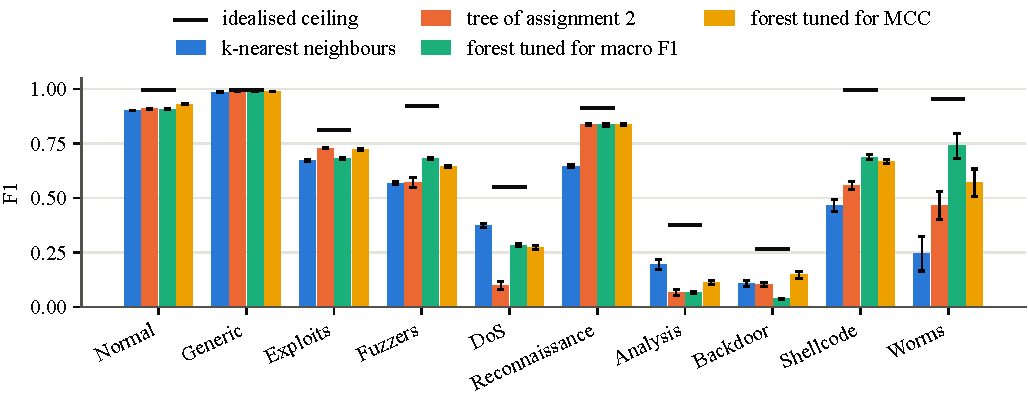
\includegraphics{figures/per_class_f1.pdf}
\caption{Per-class F1, ordered by the number of instances, with the idealised ceiling}
\label{fig:perclass}
\end{figure*}

\subsection{Sources of the Improvement}

The comparison alone does not show why the forest won. The choice of a random
forest assumed that averaging reduces the variance of the tree, so the untuned
forest was expected to outperform the tree through a lower variance.
Table~\ref{tab:bv} shows the opposite.
Both forests showed
more variance than the tree of assignment 2 over all instances, at 0.065 and 0.089
against 0.036.

\begin{table}[t]
\centering
\caption{Decomposition of the zero-one loss over all instances and as the mean over classes}
\label{tab:bv}
\footnotesize
\setlength{\tabcolsep}{2.5pt}
\begin{tabular}{lcccccc}
\toprule
& \multicolumn{3}{c}{All instances} & \multicolumn{3}{c}{Mean over classes} \\
\cmidrule(lr){2-4}\cmidrule(l){5-7}
Model & Loss & Bias & Variance & Loss & Bias & Variance \\
\midrule
Unpruned tree & 0.202 & 0.177 & 0.112 & 0.452 & 0.428 & 0.209 \\
Tree & 0.184 & 0.180 & 0.036 & 0.481 & 0.469 & 0.080 \\
Untuned forest & 0.177 & 0.174 & 0.065 & 0.469 & 0.469 & 0.130 \\
Tuned forest & 0.228 & 0.230 & 0.089 & 0.365 & 0.366 & 0.157 \\
\bottomrule
\end{tabular}
\end{table}

The cause lay in the tree rather than in the theory. On a full outer training
partition, the tree of assignment 2 had 174 leaves and a depth of 22. The same tree
without pruning had 14\,568 leaves and a depth of 58, so the tree of assignment 2
was heavily pruned. Pruning lowers the capacity of a tree and therefore yields low
variance and high bias. The argument for bagging applies to the unpruned tree
instead, and the unpruned tree therefore served as the reference for the effect of
ensembling.

The pruning had been selected on the tuning subsample. The implementation weights
the cost of each node by the proportion of training instances in the
node,\footnote{\url{https://scikit-learn.org/stable/modules/tree.html}} so the same
value of $\alpha$ prunes more on a larger training set. On an inner training fold of
32\,000 instances, $\alpha = 10^{-4}$ retained 353 of 3\,914 leaves. On an outer
training partition of about 206\,000 instances, the same value retained only 174 of
14\,568 leaves. A hyperparameter tuned on a subsample therefore did not carry the
same meaning on the full dataset.

The unpruned tree separates the two effects, as Table~\ref{tab:comparisons} shows.
Removal of the pruning raised macro-averaged F1 by 0.044 at a probability value of
$5 \times 10^{-4}$. Ensembling added nothing to macro-averaged F1, with a difference
of $-0.002$ at a probability value of 0.76. Most of the gain on the primary measure
therefore came from the absence of pruning rather than from ensembling. The pruning
was nonetheless a trade-off rather than a mistake, since the pruned tree scored
0.013 higher on the \gls{mcc} than the unpruned tree.

Figure~\ref{fig:bv} shows that the theory held against the correct reference. Over
all instances, the untuned forest lowered the variance of the unpruned tree from
0.112 to 0.065. The bias barely changed from 0.177 to 0.174, while the loss fell
from 0.202 to 0.177. Ensembling therefore raised the \gls{mcc} by 0.027 over the
unpruned tree.

\begin{figure*}[t]
\centering
\subfloat[All instances]{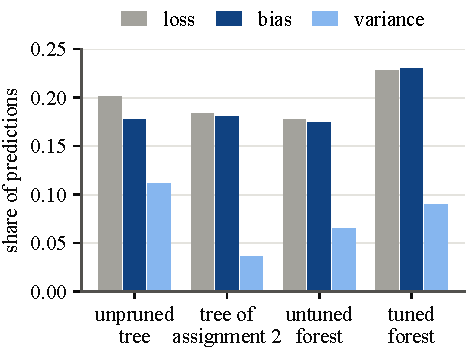
\includegraphics{figures/bias_variance_rows.pdf}}\hfill
\subfloat[Mean over classes]{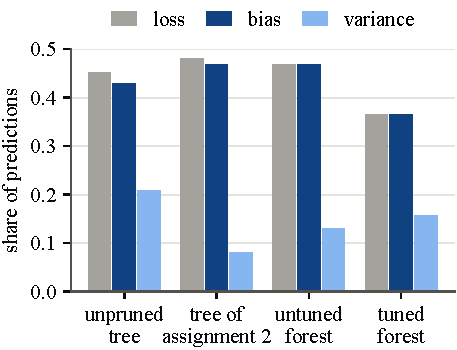
\includegraphics{figures/bias_variance_classes.pdf}}
\caption{Loss, bias and variance of the zero-one loss}
\label{fig:bv}
\end{figure*}

The mean over classes explains why macro-averaged F1 did not improve. Averaged over
classes, the bias of the forest rose from 0.428 to 0.469 and cancelled the reduction
in variance. An average of many trees converges on the majority vote, and the
majority vote favours the large class wherever a small class overlaps a large class.
A single unpruned tree is noisier, and the noise of a single tree sometimes falls on
the small class. The tuned forest lowered the mean bias over classes to 0.366
through class weighting.

\subsection{Behaviour of the Forest under Tuning}

The tuning results show whether the compared forest was well configured, and why
the selected values work. Figure~\ref{fig:trees} shows the score of the forest
against the number of trees. On the full dataset, a single tree scored 0.545. Ten
trees scored 0.583 and 100 trees scored 0.591, so most of the gain arrived within
the first 10 trees. The curve never declined, in line with the variance of an
average. The selected 100 trees made the tuned forest about seven times slower to
train than the tree, at 21 seconds per fold against three seconds.

\begin{figure}[t]
\centering
\subfloat[Tuning subsample]{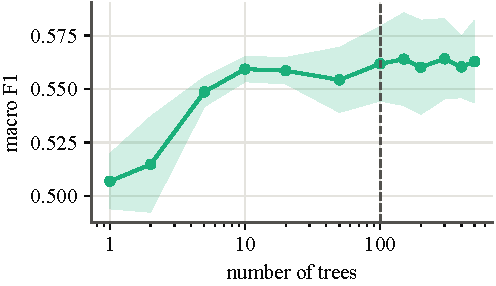
\includegraphics{figures/tree_count_inner.pdf}}\\
\subfloat[Full dataset]{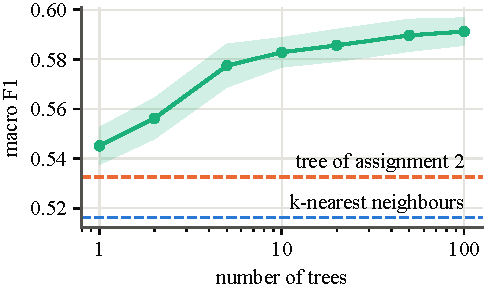
\includegraphics{figures/tree_count_outer.pdf}}
\caption{Macro-averaged F1 against the number of trees}
\label{fig:trees}
\end{figure}

Figure~\ref{fig:stage1} shows the first tuning stage. A single feature per split
scored lowest at 0.490 without weighting, and the default of six features also
scored below the best. Twenty-one features with balanced weighting scored best at
0.543, against 0.526 for all 42 features under the same weighting. Without
weighting, every value of $a$ from 10 to 42 scored between 0.523 and 0.524.
Weighting per tree scored below no weighting at every value of $a$.
Excessive randomness clearly hurt, but the advantage of moderate decorrelation over
bagging was only about one standard deviation.

\begin{figure}[t]
\centering
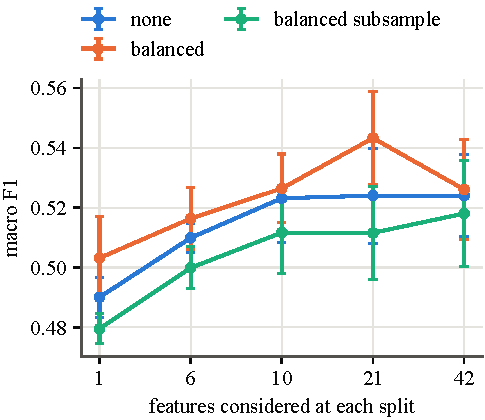
\includegraphics{figures/tuning_features_weights.pdf}
\caption{Macro-averaged F1 in the first tuning stage}
\label{fig:stage1}
\end{figure}

Figure~\ref{fig:strength} explains the shape of the first-stage curve. The mean correlation rose
with every additional feature, from 0.526 to 0.612. The strength rose quickly from
0.475 to 0.534 at 10 features before levelling off and dipping slightly at 42
features. Beyond 21 features, the trees therefore grew more alike without growing stronger.
Breiman observed the same pattern on other datasets \cite{breiman2001}. The forest score fell from 0.562 to 0.540 over that range, even though the
single trees improved from 0.500 to 0.505. The bound of Breiman exceeded one and was not informative as a bound, although the
minimum of the bound coincided with the best forest at 21 features. A moderate
number of features per split therefore balanced the strength and the correlation
of the trees.

\begin{figure*}[t]
\centering
\subfloat[Strength]{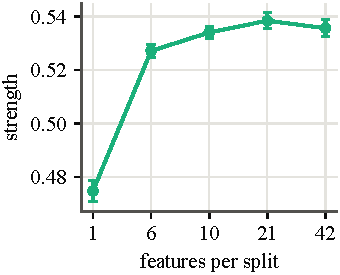
\includegraphics{figures/strength.pdf}}\hfill
\subfloat[Mean correlation]{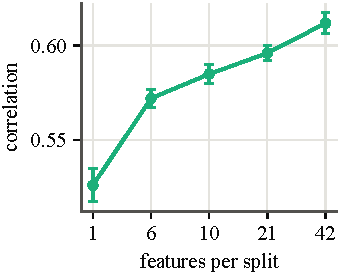
\includegraphics{figures/correlation.pdf}}\hfill
\subfloat[Macro-averaged F1]{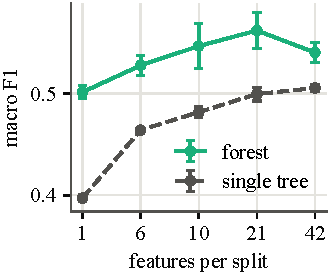
\includegraphics{figures/strength_f1.pdf}}
\caption{Strength, mean correlation and macro-averaged F1 against the number of features considered at each split}
\label{fig:strength}
\end{figure*}

The second stage favoured nearly fully grown trees. The combination of $\omega = 2$
and the entropy scored best at 0.560, while a minimum leaf size of 25 lowered the
score to 0.491. Fully grown trees suited the forest because averaging removes much
of the variance of each tree. The heavy pruning of the tree of assignment 2 is
therefore unnecessary inside a forest. The search for the \gls{mcc} preferred
larger leaves with $\omega = 10$, so the preferred size of the trees depended on the
objective.

\subsection{Class Weighting and the Tuning Objective}

The two tuned forests achieved the same macro-averaged F1 of 0.591 and 0.590, with a
probability value of 0.57 for the difference. The forest tuned for macro-averaged F1
nonetheless had the lowest accuracy of all six models at 0.771, against 0.828 for
the forest tuned for the \gls{mcc}. Class weighting explains the difference, because
the first forest used balanced weighting while the second forest used none.

Balanced weighting was selected on the strength of a single class. In the inner
cross-validation, weighting raised macro-averaged F1 by 0.019 at $a = 21$. The Worms
class gained 0.24 in F1, while the Normal and Exploits classes each lost about 0.03.
The Reconnaissance and Backdoor classes each lost about 0.04. One class contributes
one tenth of macro-averaged F1, so the Worms class alone contributed 0.024 and
exceeded the net gain. A class with 27 instances in the tuning subsample therefore
decided the weighting. The search for the \gls{mcc} counted every instance equally
and rejected weighting at every value of $a$.

Table~\ref{tab:votes} shows the cost of the weighting on the full dataset. Among the
40\,400 conflicting instances, an unweighted vote awarded 26\,332 instances to
Exploits and two to Backdoor. A vote weighted by $w_c$ awarded 136 instances to
Exploits and 20\,939 to Backdoor, because a Backdoor instance carries about 19 times
the weight of an Exploits instance. The weighted forest predicted Backdoor for
20\,591 conflicting instances and therefore reproduced the weighted vote. The
precision of the weighted forest on Backdoor fell to 0.021, while the forest tuned
for the \gls{mcc} predicted Backdoor for none of the conflicting instances.

\begin{table}[t]
\centering
\caption{Labels awarded to the 40\,400 conflicting instances}
\label{tab:votes}
\small
\begin{tabular}{lrrrr}
\toprule
Source & Exploits & Backdoor & \acrshort{dos} & Analysis \\
\midrule
Unweighted vote & 26\,332 & 2 & 8\,706 & 6 \\
Weighted vote & 136 & 20\,939 & 12\,777 & 4\,409 \\
Tree & 36\,151 & 0 & 377 & 0 \\
Untuned forest & 26\,230 & 61 & 10\,466 & 41 \\
Forest, macro F1 & 516 & 20\,591 & 9\,134 & 8\,093 \\
Forest, \acrshort{mcc} & 27\,531 & 0 & 9\,243 & 0 \\
\bottomrule
\end{tabular}
\end{table}

The weighting did buy recall on the small classes. The weighted forest detected 89.7
percent of Worms against 49.5 percent for the unweighted forest, at the cost of a
macro-averaged precision of only 0.591. The unweighted forest achieved the highest
macro-averaged precision of all six models at 0.765. The two forests therefore
reached the same macro-averaged F1 by opposite routes.

Class weighting adds no information. Between separable classes, weighting moves the
decision boundary towards the small class. Among identical instances, weighting only
changes the winning label. The cost on the large classes became visible only on the
full dataset, so the macro-averaged F1 of the tuning subsample did not reveal the
cost. The forest tuned for the \gls{mcc} is therefore preferable unless a missed
Worms attack costs more than many false positives.

\subsection{Duplicated Instances}

Duplicated instances could have distorted the comparison. About 45 percent of the
instances in each outer test fold had an exact copy in the training partition, so a
model could score well on those instances by memorisation alone. Copies with a
consistent label were indeed classified almost perfectly, with an accuracy between
0.97 and 1.00 for every model. The conflicting instances formed a third of the copies. Every model misclassified most
conflicting instances. Table~\ref{tab:duplicates}
shows that the two effects combined to lower the score of every model on the
instances with a copy. On the instances without a copy, every model scored higher.
The ranking of the models was unchanged and the gaps widened, so the duplicates do
not explain the advantage of the forest.

\begin{table*}[t]
\centering
\caption{Macro-averaged F1 on test instances with and without a copy in the training partition}
\label{tab:duplicates}
\small
\begin{tabular}{lcccccc}
\toprule
Test instances & \acrshort{knn} & Tree & Unpruned tree & Untuned forest & Forest, macro F1 & Forest, \acrshort{mcc} \\
\midrule
All & 0.516 & 0.533 & 0.577 & 0.574 & 0.591 & 0.590 \\
With a copy & 0.505 & 0.491 & 0.521 & 0.529 & 0.539 & 0.522 \\
Without a copy & 0.549 & 0.591 & 0.633 & 0.658 & 0.715 & 0.671 \\
\bottomrule
\end{tabular}
\end{table*}

In summary, the random forest outperformed both models of assignment 2 on the
primary measure and on the instances without a copy. The
absence of pruning explained most of the gain, while ensembling reduced variance and
improved the \gls{mcc} rather than macro-averaged F1. Class weighting traded overall
accuracy for the detection of the small classes, so the forest tuned for the
\gls{mcc} offered the best balance between the two measures.

%======================================================================
\section{Conclusion}
%======================================================================
\glsresetall

The study examined whether a random forest outperforms the \gls{knn} model and the
classification tree of assignment 2 in the classification of network traffic attack
categories. The random forest was chosen because the forest shares the base learner
and the pre-processing of the tree. All models were evaluated on identical
five-fold stratified partitions.

The random forest outperformed both models. The forest tuned for macro-averaged F1
exceeded the tree by 0.059 and the \gls{knn} model by 0.075 on that measure. The
forest tuned for the \gls{mcc} matched that score at an accuracy of 0.828 and was the
only model that outperformed the tree on both measures.

The supporting analyses qualified the source of the improvement. The tree of
assignment 2 was heavily pruned because the pruning parameter scales with the size
of the training set. Removal of the pruning explained most of the gain on
macro-averaged F1, while ensembling reduced variance and improved the \gls{mcc}
rather than macro-averaged F1.

The tuning showed that about 100 trees sufficed and that a moderate number of
features per split balanced the strength and the correlation of the trees. Class
weighting raised macro-averaged F1 through a single small class. The same weighting
flipped groups of identical instances to the Backdoor class and cost 5.7 percentage
points of accuracy. Conflicting instances limited every model on the \gls{dos},
Analysis and Backdoor classes.

The forest tuned for the \gls{mcc} was concluded to be the most suitable model. An
operator who must detect every Worms attack would prefer the weighted forest at the
cost of many false positives.

A few directions remain for future work. Nested cross-validation would remove the
overlap between the tuning subsample and the test folds \cite{cawley2010}. 
The forest predicts the class with the largest share of the votes. 
Scaling the share of each class by a factor tuned after training would offer an alternative to 
class weighting without retraining the forest. Bias formed most of the loss of every forest, so averaging left most of the error
untouched. Future work could compare the forest with boosting, an ensemble that targets bias rather than
variance \cite{hastie2009}. Boosting is sensitive to label noise
\cite{frenay2014}, so the comparison would also show whether the conflicting instances limit
boosting more than the forest

\bibliographystyle{IEEEtran}
\bibliography{references}
\end{document}
